% =========================================================
% CONFIGURACION DEL DOCUMENTO
% =========================================================
\providecommand{\main}{../..}
\documentclass[\main/main.tex]{subfiles}

% =========================================================
% CONTENIDO
% =========================================================
\begin{document}
\section{Simulación}\label{Simulacion}

\subsection{\noindent Estimación de los parámetros de la planta}

Para realizar una simulación lo más parecida a implementar un control
sobre la planta real, se deben calcular los parámetros físicos de
ésta, tales como las constantes de inercia, las constante de empuje
y torque de actuadores, largo de los ejes y el peso de cada componente. 


\subsubsection{Peso de componentes}

Utilizando una balanza se registra el peso de todos los componentes
del vehículo, los cuales serán utilizados para realizar el cálculo
de las inercias de rotación en cada eje. En la siguiente tabla se
registran los pesos de cada una de las partes.



\begin{table}[H]
\begin{centering}
\begin{tabular}{|c|c|c|c|}
\hline 
Componentes  & Unidades & Unidades  & Peso{[}g{]}\tabularnewline
 & Disponibles & Utilizadas & (c/u)\tabularnewline
\hline 
\hline 
Controlador myRIO & 1 & 1 & 195.6\tabularnewline
\hline 
Sendor IMU 9dof & 1 & 1 & 6.3\tabularnewline
\hline 
Power Distribution Board & 1 & 1 & 28.7\tabularnewline
\hline 
Baterías  & 2 & 1 & 516\tabularnewline
\hline 
Motores & 6 & 4 & 112.5\tabularnewline
\hline 
ESC & 6 & 4 & 32.5\tabularnewline
\hline 
Hélices  & 8 & 4 & 31.6\tabularnewline
\hline 
Brazos Fibra de Carbón & 4 & 4 & 32.2\tabularnewline
\hline 
Centro de Marco & 1 & 1 & 51.4\tabularnewline
\hline 
Apoyos de Estructura & 4 & 4 & 28.4\tabularnewline
\hline 
Protecciones & 8 & 4 & 16.4\tabularnewline
\hline 
Tren de Aterrizaje & 1 & 1 & 250\tabularnewline
\hline 
Total de Estructura & 1 & 1 & 2062.4\tabularnewline
\hline  
\end{tabular}
\par\end{centering}
\caption{Peso de las componentes del sistema.}
\end{table}

\subsubsection{Inercias para cada eje del vehículo}

Para calcular la matriz de inercias del sistema, se considera que
la estructura del vehículo es simétrica, se toma en cuenta la posición
de batería con el controlador diferenciando entre los ejes pitch y
roll, y se hace el supuesto de que los componentes poseen formas uniformes
con densidad constante.

El cálculo de los momentos de inercia se puede separar en tres partes,
mejor dicho, se pueden calcular para cada eje de rotación por separado,
bajo el supuesto de que los momentos son constantes en el tiempo independiente
de la posición y orientación del vehículo.

\begin{figure}[H]
\noindent \begin{centering}
\includegraphics[scale=0.1]{\string"inercia 2\string".jpg}\includegraphics[scale=0.1]{\string"inercia 1\string".jpg}
\par\end{centering}
\caption{Diagrama del vehículo con simplificaciones para el cálculo de Inercias.}
\end{figure}

\textbf{Eje X angulo Roll, eje Y angulo Pitch y eje Z angulo Yaw}

Para el calculo del momento de inercia sobre los ejes X (Roll) e Y
(Pitch) se toman en cuenta los siguientes supuestos:
\begin{itemize}
\item Los motores tienen forma cilíndrica de radio $R$ y altura $L$ y
masa $m$, considerando el peso de los apoyos.
\item El centro del marco del quadcopter es también cilíndrico de radio
$R$, altura $h$ y masa $m$.
\item La batería es un prisma rectangular al igual que el controlador, de
ancho $b$, alto $c$ y profundidad $a$. 
\item Sobre los brazos se considera el peso de los controladores programables
uniformemente distribuidos. También se supone una forma cilíndrica
para estas partes.
\end{itemize}

El momento de inercia sobre el eje X se calcula tomando en cuenta el efecto
de los motores 2 y 4 con un radio de giro $\ell$, los brazos del vehículo, los motores 1 y 3 que están sobre
el mismo eje y las partes centrales del marco como lo son batería,
controlador. Las expresiones para los cálculos fueron desarrolladas tomando en cuenta [14], 
junto con expresiones generales para inercias de sólidos y el teorema de los ejes paralelos.
Similarmente se calculan las inercias para el eje Y Pitch y eje Z Yaw.

\textcompwordmark{}

\begin{table}[H]
\noindent \begin{centering}
\begin{tabular}{|c|c|c|}
\hline 
\textbf{Componente } & \textbf{Expresión} & \textbf{Resultado $[Kg\cdot m^2]$}\tabularnewline
\hline 
\hline 
Motor 2 y 4 & $I_{xx}=2\cdot(\frac{mR^{2}}{4}+\frac{mh^{2}}{12}+m\ell^{2})$ & $2.60\cdot10^{-4}$\tabularnewline
\hline 
Motor 1 y 3 & $I_{xx}=2\cdot(\frac{mR^{2}}{4}+\frac{mh^{2}}{12})$ & $4.73\cdot10^{-5}$\tabularnewline
\hline 
Brazos Perpendiculares & $I_{xx}=\frac{1}{12}m\cdot(2\ell)^{2}$ & $3.16\cdot10^{-3}$\tabularnewline
\hline 
Brazos Paralelos & $I_{xx}=\frac{1}{2}mR_{b}^{2}$ & $1.8\cdot10^{-5}$\tabularnewline
\hline 
myRIO & $I_{xx}=\frac{1}{12}m\cdot(a_{mR}^{2}+c_{mR}^{2})$ & $3.15\cdot10^{-4}$\tabularnewline
\hline 
Batería & $I_{xx}=\frac{1}{12}m\cdot(a_{LiPo}^{2}+c_{LiPo}^{2})$ & $9.47\cdot10^{-4}$\tabularnewline
\hline 
Centro del Marco & $I_{xx}=\frac{mR^{2}}{4}+\frac{mh^{2}}{12}$ & $3.13\cdot10^{-5}$\tabularnewline
\hline 
\multicolumn{1}{c|}{} & \textbf{TOTAL} & $4.78\cdot10^{-3}$\tabularnewline
\cline{2-3} 
\end{tabular}
\par\end{centering}
\caption{Momento de Inercia Eje X Roll.}
\end{table}

\begin{table}[H]
\noindent \begin{centering}
\begin{tabular}{|c|c|c|}
\hline 
\textbf{Componente } & \textbf{Expresión} & \textbf{Resultado $[Kg\cdot m^2]$}\tabularnewline
\hline 
\hline 
Motor 2 y 4 & $I_{yy}=2\cdot(\frac{mR^{2}}{4}+\frac{mh^{2}}{12}+m\ell^{2})$ & $2.60\cdot10^{-4}$\tabularnewline
\hline 
Motor 1 y 3 & $I_{yy}=2\cdot(\frac{mR^{2}}{4}+\frac{mh^{2}}{12})$ & $4.73\cdot10^{-5}$\tabularnewline
\hline 
Brazos Perpendiculares & $I_{yy}=\frac{1}{12}m\cdot(2\ell)^{2}$ & $3.16\cdot10^{-3}$\tabularnewline
\hline 
Brazos Paralelos & $I_{yy}=\frac{1}{2}mR_{b}^{2}$ & $1.8\cdot10^{-5}$\tabularnewline
\hline 
myRIO & $I_{yy}=\frac{1}{12}m\cdot(b_{mR}^{2}+c_{mR}^{2})$ & $1.38\cdot10^{-4}$\tabularnewline
\hline 
Batería & $I_{yy}=\frac{1}{12}m\cdot(b_{LiPo}^{2}+c_{LiPo}^{2})$ & $1.58\cdot10^{-4}$\tabularnewline
\hline 
Centro del Marco & $I_{yy}=\frac{mR^{2}}{4}+\frac{mh^{2}}{12}$ & $3.13\cdot10^{-5}$\tabularnewline
\hline 
\multicolumn{1}{c|}{} & \textbf{TOTAL} & $3.81\cdot10^{-3}$\tabularnewline
\cline{2-3} 
\end{tabular}
\par\end{centering}
\caption{Momento de Inercia Eje Y Pitch.}
\end{table}

\begin{table}[H]
\noindent \begin{centering}
\begin{tabular}{|c|c|c|}
\hline 
\textbf{Componente } & \textbf{Expresión} & \textbf{Resultado $[Kg\cdot m^2]$}\tabularnewline
\hline 
\hline 
Motores & $I_{zz}=4\cdot(\frac{mR^{2}}{2}+m\ell^{2})$ & $0.0329$\tabularnewline
\hline 
Brazos & $I_{zz}=4\cdot\frac{1}{3}m\ell^{2}$ & $3.1298\cdot10^{-3}$\tabularnewline
\hline 
myRIO & $I_{zz}=\frac{1}{12}m\cdot(a_{mR}^{2}+b_{mR}^{2})$ & $4.321\cdot10^{-4}$\tabularnewline
\hline 
Batería & $I_{zz}=\frac{1}{12}m\cdot(a_{LiPo}^{2}+b_{LiPo}^{2})$ & $9.9489\cdot10^{-4}$\tabularnewline
\hline 
Centro del Marco & $I_{zz}=\frac{mR^{2}}{4}$ & $2.6875\cdot10^{-5}$\tabularnewline
\hline 
\multicolumn{1}{c|}{} & \textbf{TOTAL} & $3.7483\cdot10^{-2}$\tabularnewline
\cline{2-3} 
\end{tabular}
\par\end{centering}
\caption{Momento de Inercia Eje Z Yaw.}
\end{table}

\subsubsection{Caracterización de Actuadores}

Para caracterizar los actuadores se utilizó el banco de prueba Turnigy
Test Stand [15], donde se mide el empuje producido por el motor más las
hélices. Para esta prueba también fue necesario medir la velocidad
angular de giro de los actuadores, utilizando un tacómetro óptico.
Todo ésto debido a que se desea estimar la constante que relaciona
empuje con velocidad y ciclo de trabajo, mientras que la constante
que relaciona el torque de los motores es dada por el fabricante.
A continuación se muestran los gráficos que resumen la información
obtenida con las mediciones. En el Anexo C se detallan
las tablas con los datos de empuje y los entregados por el fabricante.

\textcompwordmark{}

\begin{figure}[H]
\noindent \begin{centering}
\subfloat[{Velocidad Angular {[}RPM{]} v/s empuje {[}N{]}.}]{\noindent \begin{centering}
\includegraphics[scale=0.7]{\string"RPM vs Empuje N\string".pdf}
\par\end{centering}
}\subfloat[{Velocidad Angular {[}RPM$^{2}${]} v/s Empuje {[}N{]}.}]{\noindent \begin{centering}
\includegraphics[scale=0.7]{\string"RPM2 vs empuje N\string".pdf}
\par\end{centering}}
\par\end{centering}
\noindent \begin{centering}
\subfloat[{Velocidad Angular {[}Rad/s{]} v/s Empuje {[}N{]}.}]{\noindent \begin{centering}
\includegraphics[scale=0.7]{\string"RadS vs Empuje N\string".pdf}
\par\end{centering}
}\subfloat[{Velocidad Angular {[}Rad/s$^{2}${]} v/s Empuje {[}N{]}}]{\noindent \begin{centering}
\includegraphics[scale=0.7]{\string"RadS2 vs Empuje N\string".pdf}
\par\end{centering}}
\par\end{centering}
\caption{Mediciones de Velocidad Angular v/s Empuje.}
\end{figure}

\textcompwordmark{}

En la siguiente tabla se resumen las constantes de proporcionalidad
entre velocidad angular versus empuje. 

\begin{table}[H]
\noindent \begin{centering}
\begin{tabular}{|c|c|c|}
\hline 
Actuador & Parámetro k$_1$ {[}N/(Rad/s)$^{2}${]} & Parámetro k$_2$ {[}N/(Rad/s) {]}\tabularnewline
\hline 
\hline 
1 & $1.6276\cdot10^{-5}$ & $1.9210\cdot10^{-5}$\tabularnewline
\hline 
2 & $1.4578\cdot10^{-5}$ & $2.0423\cdot10^{-5}$\tabularnewline
\hline 
3 & $1.4830\cdot10^{-5}$ & $1.9540\cdot10^{-5}$\tabularnewline
\hline 
4 & $1.3563\cdot10^{-5}$ & $1.9343\cdot10^{-5}$\tabularnewline
\hline 
\end{tabular}
\par\end{centering}
\caption{Parámetros de empuje y torque en actuadores.}
\end{table}

La constante de proporcionalidad de torque con velocidad angular es
$b=2\cdot10^{-7}[Nm/(Rad/s)^{2}]$. El gráfico liberado por el fabricante de torque v/s RPM
para baterías de 3 y 4 celdas se adjunta en el Anexo C.

Para la implementación en la simulación se considera el supuesto de
que todos los motores poseen los mismos parámetros de empuje y torque
en su caracterización, considerando el promedio lineal de los parámetros
obtenidos en el primer caso y el dato obtenido del gráfico porporcionado
por el fabricante en el último.

\textcompwordmark{}

\subsection{Resultados de la simulación}

En esta sección se presentan los resultados al simular el modelo no lineal del vehículo, controlado con la estrategia desarrollada
en el capítulo anterior. Dicho de otro modo, se toma el modelo multivariable,
no lineal y acoplado del quadrotor y se implementa una estrategia
de control lineal, como lo son los controladores de la familia PID
antes descritos.

Para la simulación se controla cada eje por separado, implementando
un controlador PD descentralizado para los ejes de rotación, como
así también para mantener el vehículo en una referencia de altura
fija. 

Cabe mencionar que los controladores son re-sintonizados en esta etapa
para lograr un mejor desempeño y robustez a pequeñas perturbaciones.
Ésto debido a las simplificaciones que se realizaron para diseñar
el control lineal de la planta. De todas formas los valores obtenidos
en la etapa de diseño entregan un buen punto de partida para la re-sintonización.

\subsubsection{Estabilización con orientación de partida inestable}

En esta prueba se libera el vehículo en una posición inicial aleatoria
e inestable dentro de los rangos permitidos. Posteriormente se logra
la estabilización del mismo manteniendo una altura constante de 4{[}m{]}.
El controlador escogido para esta prueba es un PD con filtro derivativo
de primer orden, mientras que para el control de altura se implementa
el controlador PD sugerido en el capítulo anterior. Es importante destacar
que el controlador PD para la estabilización es igual para los tres
ejes, dada la similitud en la estructura de la planta y las constantes
de inercia. La diferencia mayor es en el control de el ángulo yaw,
dada la diferencia de un orden de magnitud en la constante de inercia
respecto a los otros dos ángulos pitch y roll.

\begin{table}[H]
\noindent \begin{centering}
\begin{tabular}{|c|c|c|c|c|}
\hline 
Parámetros & $K_{p}$ & $K_{d}$ & $K_{i}$ & $\alpha$\tabularnewline
\hline 
\hline 
$\theta,\phi,\psi$ & 40 & 10 & 0 & 100\tabularnewline
\hline 
$z$ & 8 & 5 & 0 & 0\tabularnewline
\hline 
\end{tabular}
\par\end{centering}
\caption{Parámetros para los controladores.\label{tab:kp kd ki alpha}}
\end{table}

A continuación se presentan los gráficos de la simulación partiendo por el desplazamiento angular y velocidad angular en los ejes del vehículo, la altura de éste y por último la actuación en porcentaje de ciclo de trabajo de la señal PWM de los motores.

\begin{figure}[H]
\noindent \begin{centering}
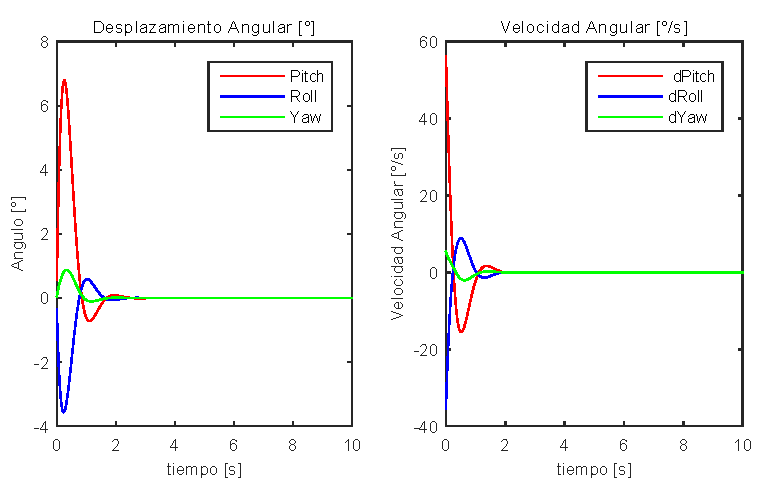
\includegraphics[scale=0.8]{Estabilizacion1}
\par\end{centering}
\caption{Control PD descentralizado para estabilización en hovering sin perturbación,
altura 4{[}m{]}.}
\end{figure}

\begin{figure}[H]
\noindent \begin{centering}
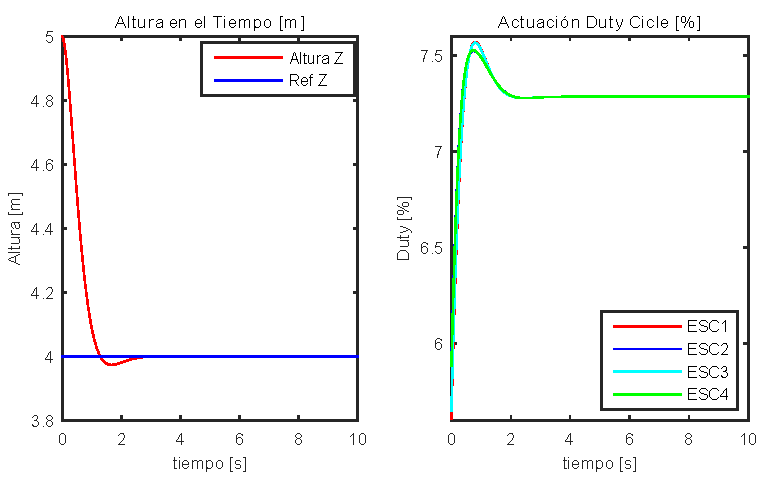
\includegraphics[scale=0.8]{Estabilizacion11}
\par\end{centering}
\caption{Seguimiento de altura y actuación en el tiempo.}
\end{figure}

\subsubsection{Estabilización partida inestable con perturbación en Pitch}

En esta prueba se libera el vehículo en una posición aleatoria e inestable
dentro de los rangos permitidos. Posteriormente se logra la estabilización
y seguimiento de altura. En seguida se introduce una perturbación
al sistema simulando un empuje externo en uno de los ejes. Lo anterior
se simula modificando la velocidad de los motores 1 y 3 manualmente
por un lapso de tiempo, es decir se deja el eje pitch en lazo abierto
mientras se introduce la perturbación. El resultado obtenido manteniendo
el controlador de la tabla \ref{tab:kp kd ki alpha} es el siguiente:

\begin{figure}[H]
\noindent \begin{centering}
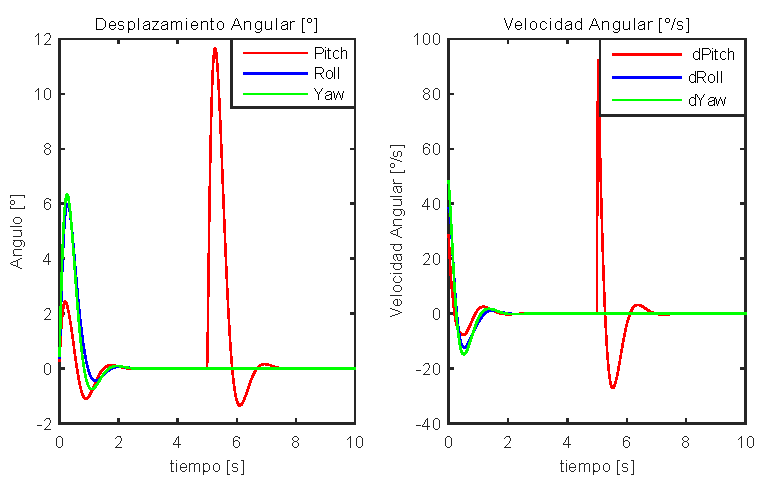
\includegraphics[scale=0.8]{Estabilizacion2}
\par\end{centering}
\caption{Control PD descentralizado para estabilización con perturbación en Pitch.}
\end{figure}

\begin{figure}[H]
\noindent \begin{centering}
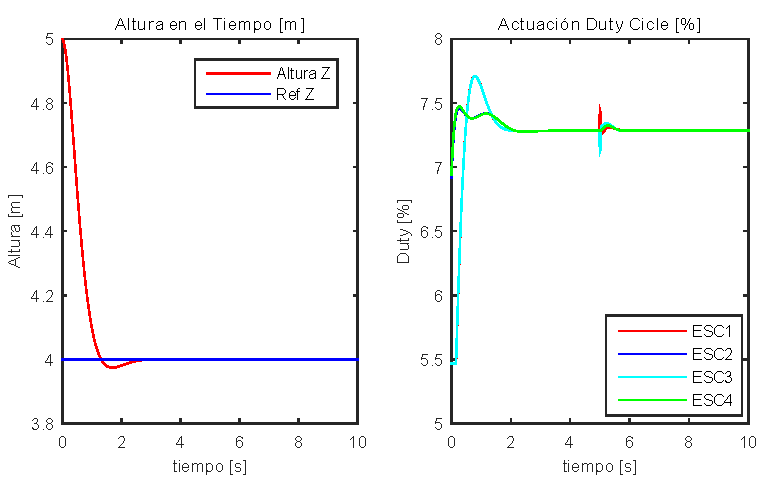
\includegraphics[scale=0.8]{Estabilizacion22}
\par\end{centering}
\caption{Seguimiento de altura y Actuación en el tiempo.}
\end{figure}

\begin{figure}[H]
\noindent \begin{centering}
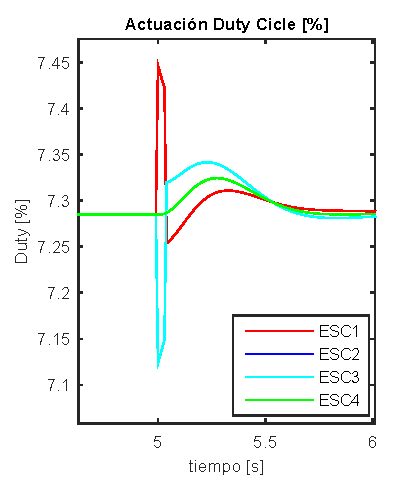
\includegraphics[scale=0.8]{Estabilizacion221}
\par\end{centering}
\caption{Acercamiento actuación al introducir perturbación.}
\end{figure}

\subsubsection{Estabilización partida inestable con perturbación en Roll}

Luego de liberar el vehículo con la misma lógica que en los puntos
anteriores, se introduce una perturbación en el eje Roll, con la misma
estrategia utilizada en Pitch, pero esta vez modificando la velocidad
de los motores 2 y 4, manteniendo el mismo controlador.

\begin{figure}[H]
\noindent \begin{centering}
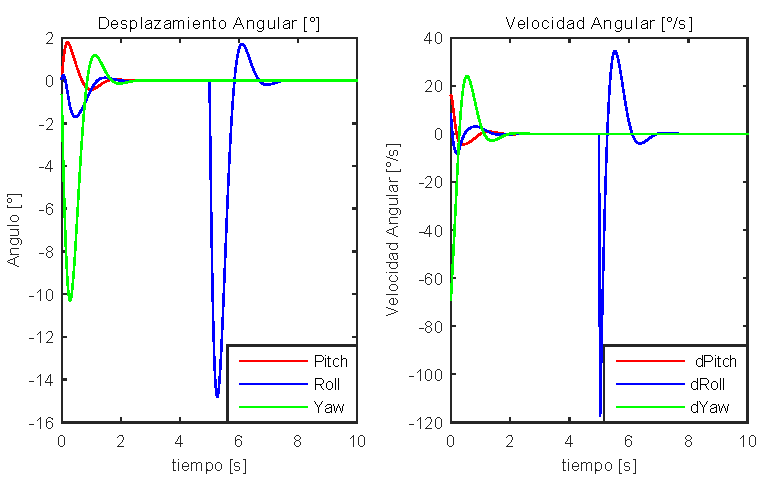
\includegraphics[scale=0.8]{Estabilizacion3}
\par\end{centering}
\caption{Control PD descentralizado para estabilización con perturbación en Roll.}
\end{figure}

\begin{figure}[H]
\noindent \begin{centering}
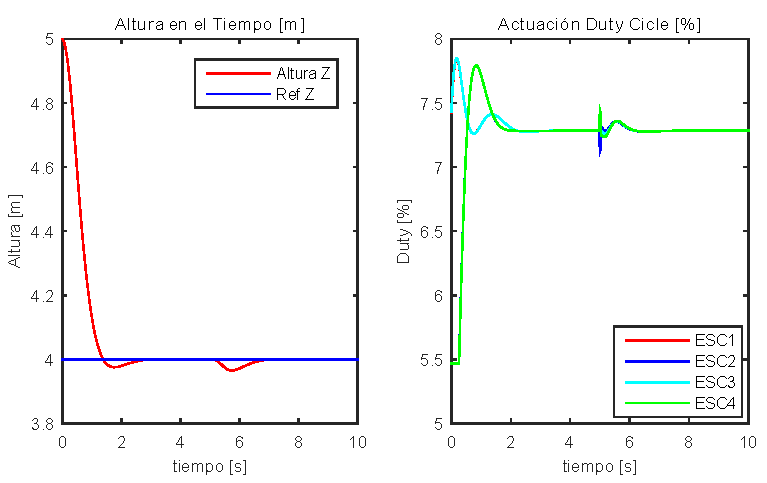
\includegraphics[scale=0.8]{Estabilizacion33}
\par\end{centering}
\caption{Seguimiento de altura y actuación en el tiempo.}
\end{figure}

\begin{figure}[H]
\noindent \begin{centering}
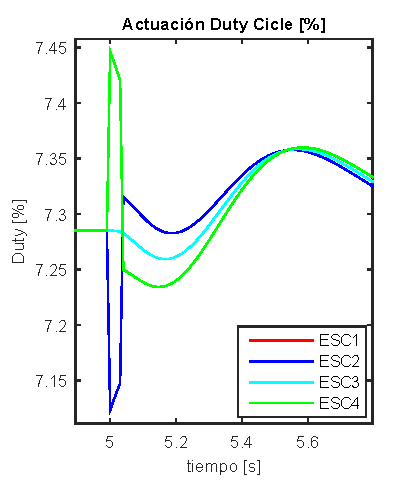
\includegraphics[scale=0.8]{Estabilizacion331}
\par\end{centering}
\caption{Acercamiento actuación al introducir perturbación.}
\end{figure}

\subsubsection{Estabilización partida inestable con perturbación en Yaw}

Siguiendo los mismos pasos anteriores para la partida, esta vez se
introduce una perturbación en el eje de giro yaw. La perturbación
se simula modificando la posición yaw del vehículo a velocidad constante
de 50 {[}$\degree/s${]}, puesto que si se sigue la estrategia
de modificar la velocidad de los 4 motores, se pierde el seguimiento
de altura de forma abrupta. Se mantiene el controlador y el resultado
del experimento es el siguiente:

\begin{figure}[H]
\noindent \begin{centering}
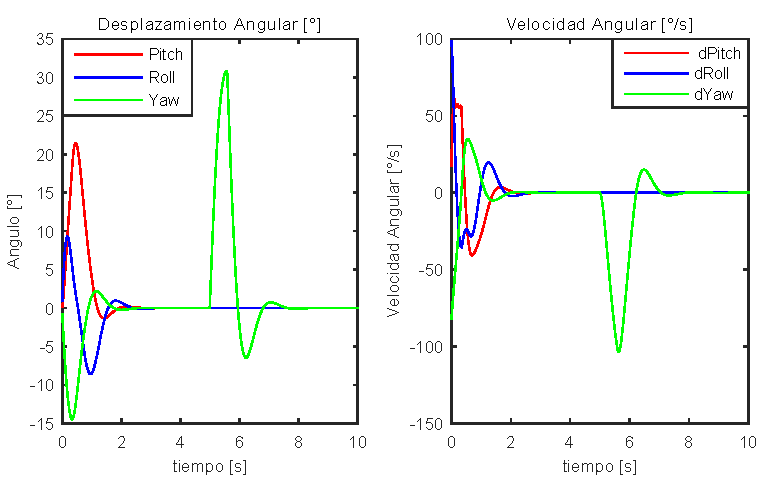
\includegraphics[scale=0.8]{Estabilizacion4}
\par\end{centering}
\caption{Control PD descentralizado para estabilización con perturbación enYaw.}
\end{figure}


\begin{figure}[H]
\noindent \begin{centering}
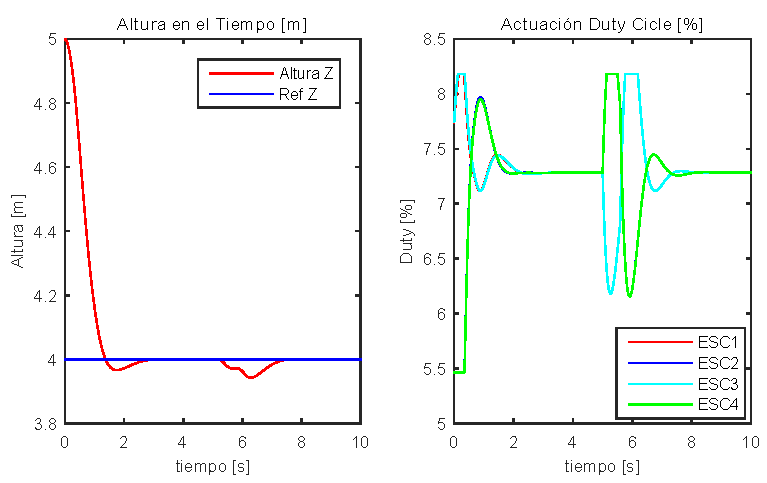
\includegraphics[scale=0.8]{Estabilizacion44}
\par\end{centering}
\caption{Seguimiento de altura y actuación en el tiempo.}
\end{figure}

\begin{figure}[H]
\noindent \begin{centering}
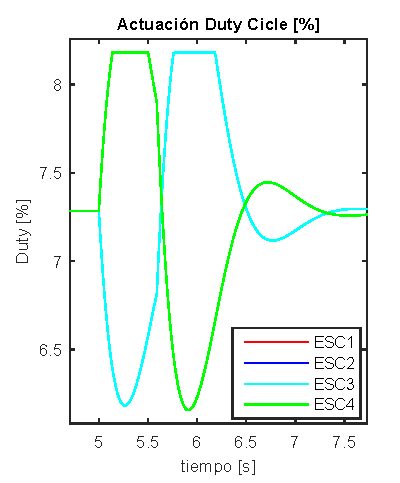
\includegraphics[scale=0.8]{Estabilizacion441}
\par\end{centering}
\caption{Acercamiento actuación al introducir perturbación.}
\end{figure}

\subsubsection{Estabilización partida inestable con perturbación en Pitch y Roll
simultáneamente}

En esta prueba se perturba el sistema en dos ejes simultáneamente
en sentido contrario a las pruebas anteriores de Pitch y Roll. La
estrategia para perturbar el sistema es similar pero esta vez modificando
la velocidad de los cuatro motores a la vez, sin variar el controlador.

\begin{figure}[H]
\noindent \begin{centering}
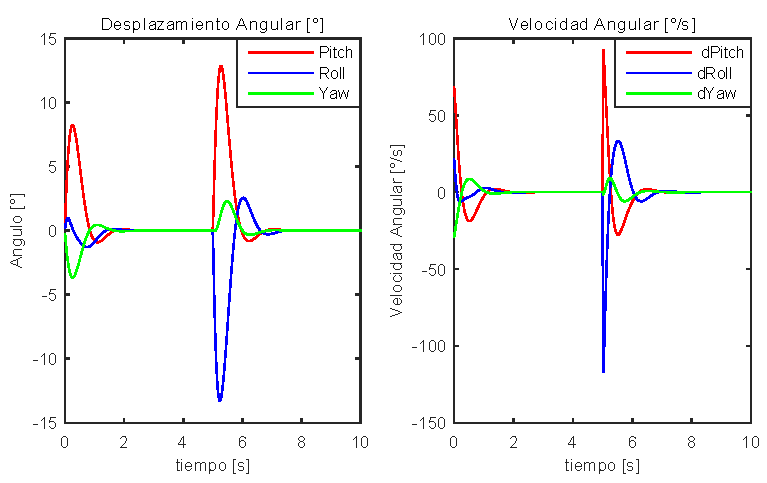
\includegraphics[scale=0.8]{Estabilizacion5}
\par\end{centering}
\caption{Control PD descentralizado para estabilización con perturbación en
Pitch y Roll simultáneamente.}
\end{figure}


\begin{figure}[H]
\noindent \begin{centering}
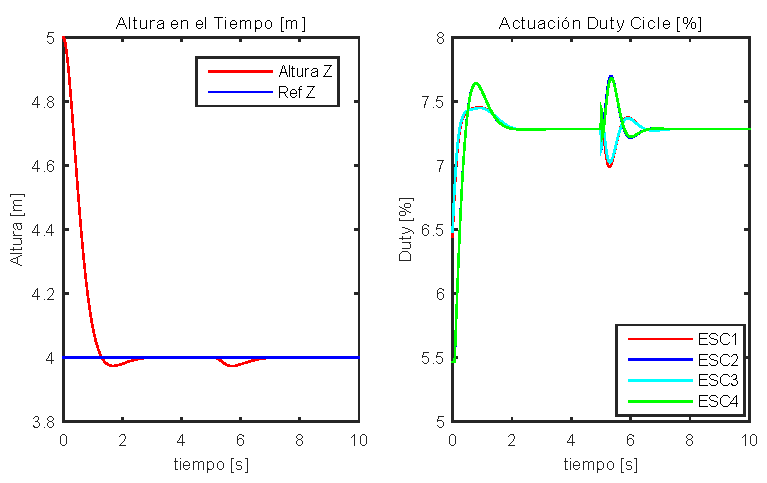
\includegraphics[scale=0.8]{Estabilizacion55}
\par\end{centering}
\caption{Seguimiento de altura y actuación en el tiempo.}
\end{figure}

\begin{figure}[H]
\noindent \begin{centering}
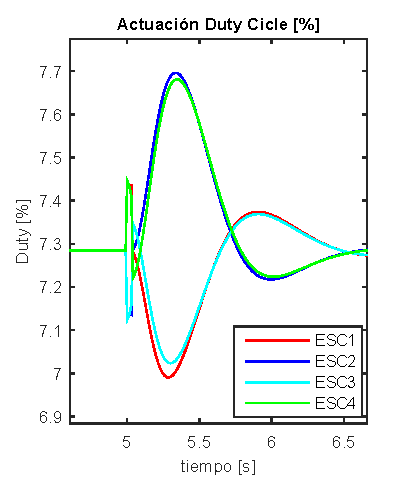
\includegraphics[scale=0.8]{Estabilizacion551}
\par\end{centering}
\caption{Acercamiento actuación al introducir perturbación.}
\end{figure}

\subsubsection{Seguimiento ángulo Pitch y Altura}

En esta sección se pone a prueba el seguimiento de referencias constantes
para cada uno de los ejes, partiendo por el eje de elevación Pitch,
controlando la altura del vehículo y monitoreando las velocidades
de giro al igual que en los casos anteriores.

\begin{figure}[H]
\noindent \begin{centering}
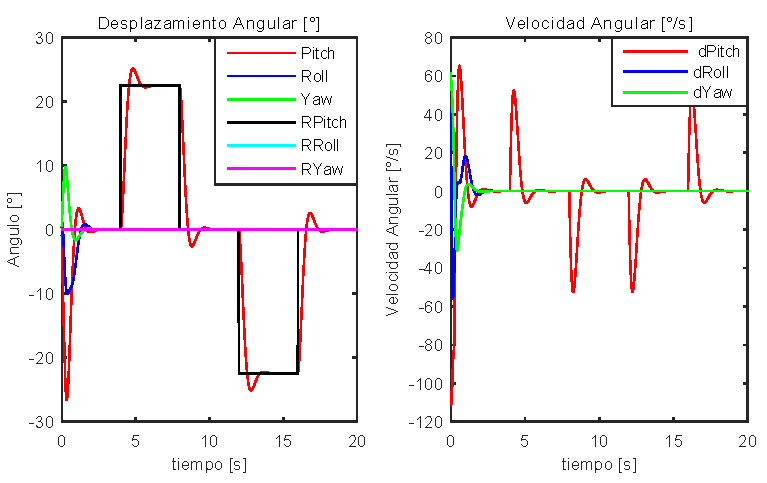
\includegraphics[scale=0.8]{Seguimiento1}
\par\end{centering}
\caption{Estabilización y seguimiento de angulo Pitch. $Referencia=\pm22.5\degree$.}
\end{figure}

\begin{figure}[H]
\noindent \begin{centering}
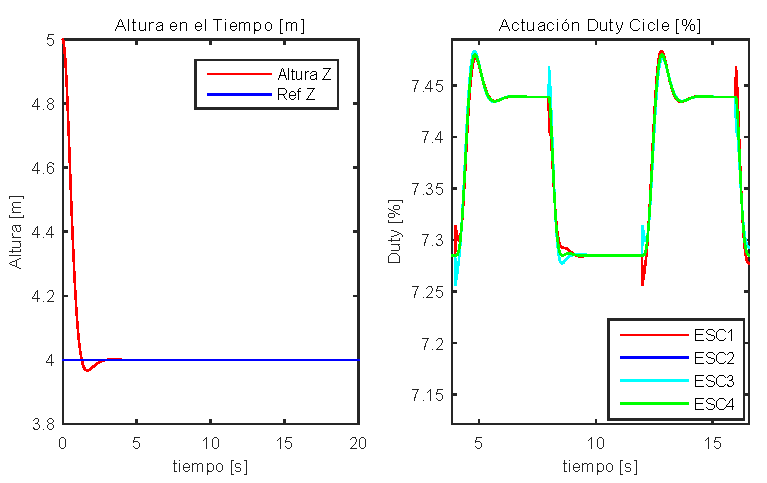
\includegraphics[scale=0.8]{Seguimiento11}
\par\end{centering}
\caption{Seguimiento de altura y actuación en el tiempo.}
\end{figure}

\subsubsection{Seguimiento angulo Roll y Altura}

En este caso se somete a prueba el seguimiento para el eje de rotación
Roll. A diferencia del caso anterior, al introducir la perturbación
al sistema la altura del vehículo tiende a disminuir, para luego ajustarse
por medio del control propio. Esto es diferente para cada eje debido
a que son constantes de inercia diferentes para cada eje, pero ambos
están estabilizados con el mismo controlador.

\begin{figure}[H]
\noindent \begin{centering}
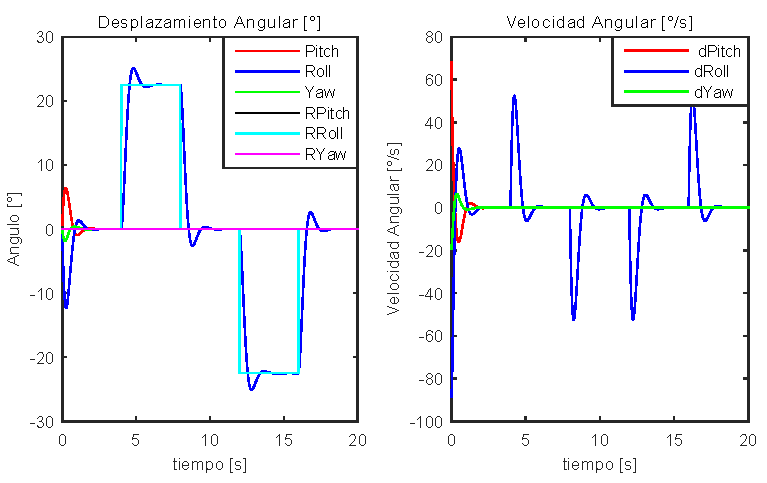
\includegraphics[scale=0.8]{Seguimiento2}
\par\end{centering}
\caption{Estabilización y seguimiento de angulo Roll. $Referencia=\pm22.5\degree.$ }
\end{figure}

\begin{figure}[H]
\noindent \begin{centering}
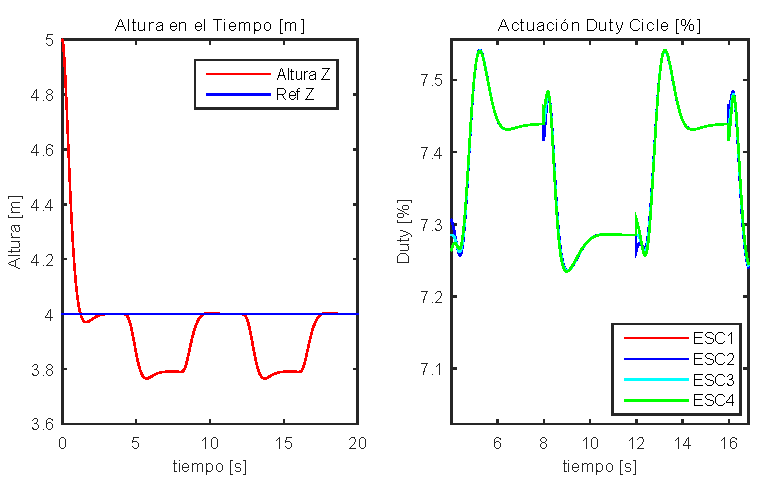
\includegraphics[scale=0.8]{Seguimiento22}
\par\end{centering}
\caption{Seguimiento de altura y actuación en el tiempo.}
\end{figure}

\subsubsection{Seguimiento Yaw y corrección de altura}

En este experimento se introduce un cambio de referencia en el eje
de rotación Yaw. A diferencia de los dos casos anteriores, se produce
un mayor número de perturbaciones en la altura del vehículo. Ésto
debido a que para controlar el giro en Yaw se alteran las velocidades
de los 4 motores, disminuyendo el empuje total al frenar el movimiento
después de cada cambio de referencia.

\begin{figure}[H]
\noindent \begin{centering}
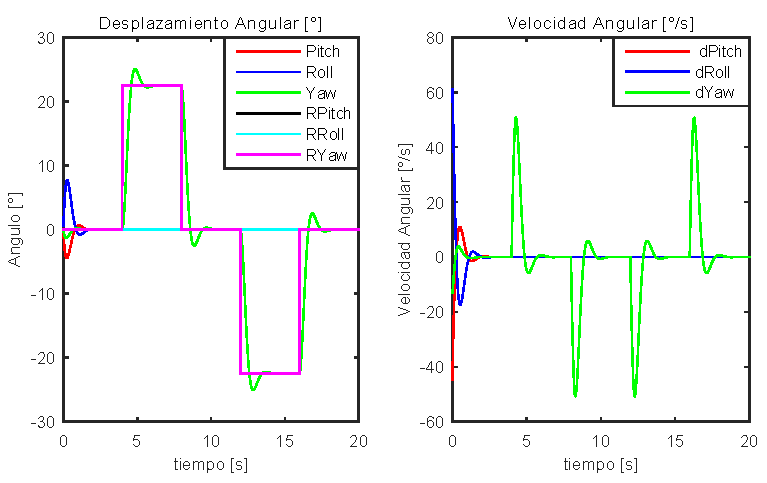
\includegraphics[scale=0.8]{Seguimiento3}
\par\end{centering}
\caption{Estabilización y seguimiento de angulo Yaw. $Referencia=\pm45\degree.$}
\end{figure}

\begin{figure}[H]
\noindent \begin{centering}
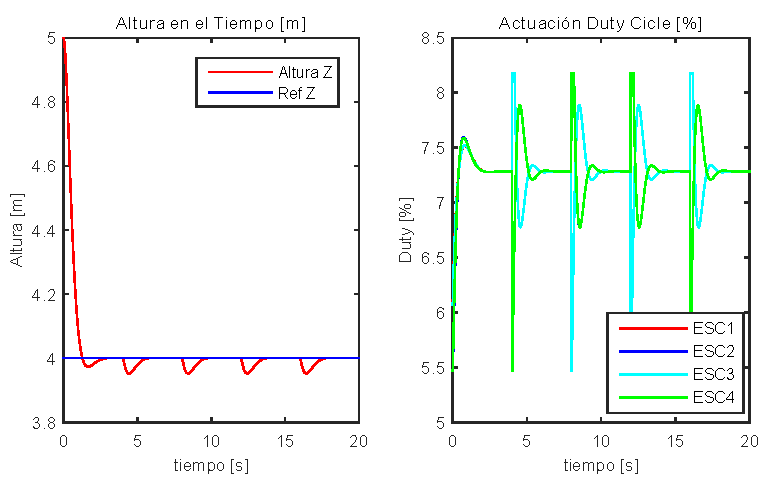
\includegraphics[scale=0.8]{Seguimiento33}
\par\end{centering}
\caption{Seguimiento de altura y actuación en el tiempo.}
\end{figure}

\subsection{Conclusiones}

Después de simular el sistema con el modelo no lineal de la planta y la
estrategia de control PID descentralizado, se puede concluir que
para la implementación un control estabilizador PD es un buen punto
de partida.

Es importante mencionar que la simulación del sistema no cuenta con
ruido de medición, por lo cual es una simulación ideal del sistema,
dado que el funcionamiento de los motores induce vibraciones sobre
la estructura, lo que se verá reflejado en la adquisición de las señales
del acelerómetro y gyróscopo. Lo anterior puede ser una limitante
para el control bajo el diseño definido.

Es importante también tener en cuenta que el soporte, mostrado en el capítulo de Componentes para la Implementación, que se utilizará
para la estabilización cambiará el modelo de la planta, puesto que
los ejes de rotación del vehículo fijado al soporte no pasan por su
centro de masa como el modelo utilizado en simulación lo supone.

\end{document}